% !TEX TS-program = pdflatex
% !TEX encoding = UTF-8 Unicode

% This is a simple template for a LaTeX document using the "article" class.
% See "book", "report", "letter" for other types of document.

\documentclass[11pt]{article} % use larger type; default would be 10pt

\usepackage[english]{babel}
\usepackage[utf8]{inputenc} % set input encoding (not needed with XeLaTeX)
\usepackage{fvextra}
\usepackage{csquotes}

%%% Examples of Article customizations
% These packages are optional, depending whether you want the features they provide.
% See the LaTeX Companion or other references for full information.

%%% PAGE DIMENSIONS
\usepackage[a4paper, top=2cm, bottom=2.2cm, left=3cm, right=3cm, includeheadfoot, headheight=31pt,
  headsep=0pt]{geometry} % to change the page dimensions
\geometry{a4paper} % or letterpaper (US) or a5paper or....
\usepackage{multicol}
\setlength{\headheight}{35pt}
\setlength{\parindent}{0pt}
% \geometry{landscape} % set up the page for landscape
%   read geometry.pdf for detailed page layout information

\usepackage{graphicx} % support the \includegraphics command and options
\usepackage[colorlinks=true, allcolors=blue]{hyperref}
\usepackage{xcolor} % Allow coloring of text.

% \usepackage[parfill]{parskip} % Activate to begin paragraphs with an empty line rather than an indent

%%% PACKAGES
\usepackage{booktabs} % for much better looking tables
\usepackage{array} % for better arrays (eg matrices) in maths
\usepackage{paralist} % very flexible & customisable lists (eg. enumerate/itemize, etc.)
\usepackage{fancyvrb} % adds environment for commenting out blocks of text & for better verbatim
\usepackage{subfig} % make it possible to include more than one captioned figure/table in a single float
\usepackage{float}
\usepackage{biblatex}[style=ieeetr]
\usepackage{parskip}
\usepackage{amsmath, amsthm, amssymb, amsfonts}
\usepackage{lipsum}
\usepackage{tabularx}
\usepackage{calculator}
% These packages are all incorporated in the memoir class to one degree or another...

% Changes date format to YYYY-MM-DD
\usepackage[yyyymmdd]{datetime}
\settimeformat{hhmmsstime}
\renewcommand{\dateseparator}{-}

% Add version number variable.
\newcounter{versionNumber}
\makeatletter
% At the end write the current value back to the `.aux` file
\AtEndDocument{
  \immediate\write\@auxout{
    \string\setcounter{versionNumber}{\number\value{versionNumber}}
  }
}
\makeatother
% Step the counter at the beginning
\AtBeginDocument{
  \stepcounter{versionNumber}
}

% Title page info
\title{Rotating Index Load Balancer Documentation}
\author{Lani Wagner\\\href{mailto:lani.wagner@students.fhnw.ch}{lani.wagner@students.fhnw.ch}}
\date{\today\ \currenttime} % Activate to display a given date or no
% otherwise the current date is printed

% Define constants to use throughout document
\makeatletter
\let\thisauthor\@author
\makeatother

%%% HEADERS & FOOTERS
\usepackage{lastpage}
\usepackage{fancyhdr} % This should be set AFTER setting up the page geometry
\pagestyle{fancy} % options: empty , plain , fancy
\renewcommand{\headrulewidth}{0pt} % customise the layout...
\lhead{}
\chead{}
\rhead{
\includegraphics[height=0.88\headheight]{res/fhnw_ht_10mm.eps}}
\lfoot{v0.0.\theversionNumber\ \textcolor{gray}{\today\ \currenttime}}
\cfoot{Lani Wagner}
\rfoot{\thepage\ /
    {\hypersetup{hidelinks}\pageref{LastPage}}}

%%% SECTION TITLE APPEARANCE
\usepackage{sectsty}
\allsectionsfont{\sffamily\mdseries\upshape} % (See the fntguide.pdf for font help)
% (This matches ConTeXt defaults)

%%% ToC (table of contents) APPEARANCE
\usepackage[nottoc]{tocbibind} % Put the bibliography in the ToC
\usepackage[titles,subfigure]{tocloft}
\usepackage{amssymb} % Alter the style of the Table of Contents
\renewcommand{\cftsecfont}{\rmfamily\mdseries\upshape}
\renewcommand{\cftsecpagefont}{\rmfamily\mdseries\upshape} % No bold!

% Change second level of enumerated lists to arabic numbers.
\renewcommand{\labelenumii}{\arabic{enumi}.\arabic{enumii}}

% Reduce spacing in whole document to compact document
\usepackage{titlesec}
\usepackage{amsfonts}
\usepackage{enumitem}% http://ctan.org/pkg/enumitem
\setlist[itemize]{noitemsep, topsep=0pt}

\newcommand{\rilb}{Rotating Index Load Balancer }
\newcommand{\hidelinks}[1]{{\hypersetup{hidelinks}#1}}
\newcommand{\figref}[1]{\hidelinks{\hyperref[#1]{Figure \ref{#1}}}}

%%% END Article customizations

%%% The "real" document content comes below...

\begin{document}
  \begin{titlepage}
    \begin{center}
      \vspace*{1cm}

      \textbf{\Huge \rilb}

      \vspace{1.5cm}
      \hrule
      \vspace{1cm}

      {\Large Documentation}

      \vspace{2.5cm}


      \begin{figure}[H]
        \centering
        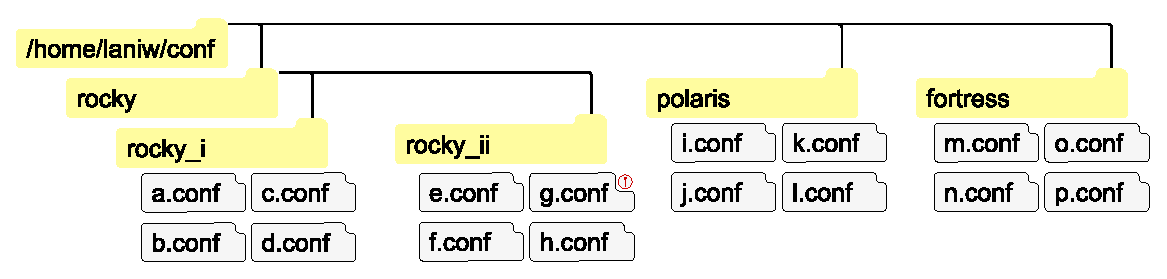
\includegraphics[width=.9\linewidth, keepaspectratio]{res/rilb_visualization}
        \label{fig:rilb-vis-title}
      \end{figure}

      \vfill

      
\includegraphics[width=0.4\textwidth]{res/fhnw_ht_10mm}

      \vspace{0.8cm}

      Lani Wagner

      \today\ \currenttime

    \end{center}
  \end{titlepage}

  \section*{Introduction}

  This document serves as a documentation for the written implementation of a rotating index load balancer as described in the pre-production specification found at \url{https://github.com/laniwfhnw/engw_specification/blob/main/engw_specification.pdf}.

    {\hypersetup{hidelinks} \tableofcontents}
  \newpage



  \section{\rilb Concept}\label{sec:2}

  To explain what the idea of a \rilb is, it's easiest to first explain what problem it solves with a simple example. Imagine a filesystem like the one shown in \figref{fig:rilb-vis}. We want to provide a service that accepts analysis requests. These analysis requests are run over the system to calculate a result. The result is then returned to the requester. You can imagine this service being an API, so we don't know when or how many of the requests we're going to get.

  The simplest solution, once we get a request, would be to go through all of the files for one request and complete the analysis. Once all of the files have been included in the result we return the result. This works fine when we don't have many requests coming in and the analyses don't need a long time to complete. We are doing a lot of the same operations multiple times, though. Every time we read a file for one analysis and then another and then another we are doing the same operation. If they come in at a similar time we can read the file once to avoid expensive I/O operations.

  The idea of reducing the amount of read operations $m \cdot n$, where $m$ is the amount of analyses that need to read $n$ files, to $n$ read operations is the main idea of a \rilb. Imagine an index that points to a file at all times and rotates around pointing to all files in the filesystem. Every time it points to a file it reads that file and passes that data on to the analyses. Once a request reaches the service, it keeps track of the first file that service received. That way the service knows the analysis has looked at all files when the index points to the file that the analysis started with.

  Let me me walk you through an example execution using the filesystem in \figref{fig:rilb-vis}. We are working with 16 different configuration files. We want to analyze these files in three different ways. The first analysis $A_1$ would like to know the average length of the files in lines. The second analysis $A_2$ would like to know what the longest line in any of the files is. Finally, the third $A_3$ analysis would like to know the size of the files in bytes that are two levels deeper than the root. At first the service isn't doing anything because there are no active analyses running. Once the first analysis $A_1$ is requested, the index starts rotating and the filecontents are analysed per analysis $A_1$. The files \texttt{a.conf}, \texttt{b.conf}, \texttt{c.conf}, and \texttt{d.conf} are analysed without any other requests coming in. Analysis $A_2$ arrives right before the index points to \texttt{e.conf}, so \texttt{e.conf} is the first file $A_2$ analyses. $A_3$ comes in when the index points to \texttt{g.conf}. The contents of \texttt{g.conf} and \texttt{h.conf} are sent to all three analyses. The files \texttt{i.conf} through \texttt{p.conf} are only sent to analyses $A_1$ and $A_2$, since analysis $A_3$ doesn't care about those files. As soon as the index points to \texttt{a.conf} the second time the service knows that analysis $A_1$ has been completed and it returns the result. The rotation continues without interruption until the index points to \texttt{e.conf}, at  which point analysis $A_2$ is returned. Now only analysis $A_3$ remains. It is still around the receive the file contents of \texttt{e.conf} and \texttt{f.conf}. The result of analysis $A_3$ is returned as soon as the index points to \texttt{g.conf}. Now there are no more analyses in the queue, so the index rests at \texttt{g.conf} until another request arrives. The  final state of the service is depicted in \figref{fig:rilb-vis}.

  \begin{figure}[H]
    \centering
    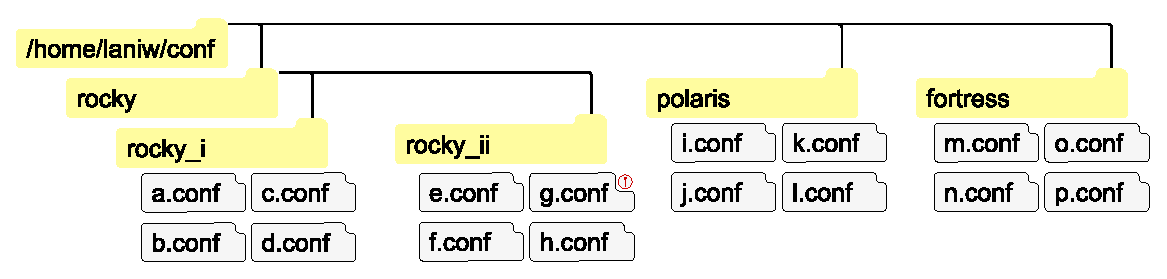
\includegraphics[width=.99\linewidth, keepaspectratio]{res/rilb_visualization}
    \caption{Visualization of a \rilb traversion through an example filesystem.}
    \label{fig:rilb-vis}
  \end{figure}

  This example obviously doesn't illustrate what happens in certain special cases. For example we didn't consider the case that \texttt{g.conf} could get deleted during the rotation of $A_3$, so with our current approach we would not know when to stop. For more detail on the exact implementation and how special cases are handled please take a look at the pre-production specification of the library\footnote{\url{https://github.com/laniwfhnw/engw_specification/blob/main/engw_specification.pdf}}.



  \section{Library Use}\label{sec:3}

  % specify how a developer can use the capabilities of the library


  \subsection{Environment}\label{sec:3.1}

  % explain on what hardware and OS the library is intended to run on


  \subsection{Use Cases}\label{sec:3.2}

  % explain for what use cases this library should be used.



  \newpage



  \section{Glossary}

  \begin{table}[H]
    \centering
    \begin{tabular}{p{.3\linewidth} | p{.6\linewidth}}
      \textbf{Term} & \textbf{Definition}
      \\\hline
      Rotation      & A single go around the list of files considered for analysis.
    \end{tabular}
    \caption{Glossary definitions.}
    \label{tab:glossary}
  \end{table}

  \printbibliography[heading=bibintoc]
  \listoffigures
  \listoftables
\end{document}